\documentclass[10pt]{article}
\usepackage{amsmath,textcomp,amssymb,geometry,graphicx,enumerate,tikz,algorithm,algpseudocode,pifont,upgreek}
\usetikzlibrary{calc}
\usetikzlibrary{datavisualization}
\usetikzlibrary{datavisualization.formats.functions}


\textheight=9in
\textwidth=7in
\topmargin=-.75in
\oddsidemargin=-0.25in
\evensidemargin=-0.25in

\usepackage{listings}
\lstnewenvironment{codeblock}
    {\lstset{language=Python,
      showspaces=false,
      showtabs=false,
      breaklines=true,
      mathescape=true,
      showstringspaces=false,
      breakatwhitespace=true,
      commentstyle=\textit,
      keywordstyle=\textbf,
      basicstyle=\ttfamily,
      escapechar=`,
    }}
    {}

\newcommand{\bigo}{\mathcal{O}}
\newcommand{\R}{\mathbb{R}}


\begin{document}
\section*{04/20/2016}
\subsection*{Clustering w/Multiple Eigenvectors}
\begin{itemize}
	\item For $k$ clusters, compute first $k$ eigenvectors $v_{1} = \textbf{1}, v_{2}, \dots, v_{k}$ of generalized eigensystem $Lv = \lambda Mv$.
		\begin{center}
			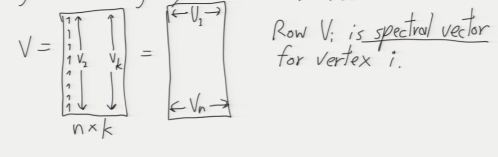
\includegraphics[scale=0.8]{../images/spectralspace}
		\end{center}
	\item Normalize each row $V_{i}$ to unit length.
		\begin{center}
			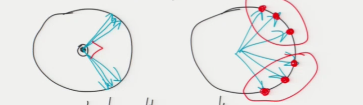
\includegraphics{../images/vectorclusters}
		\end{center}
	\item k-means cluster these vectors.
		\begin{center}
			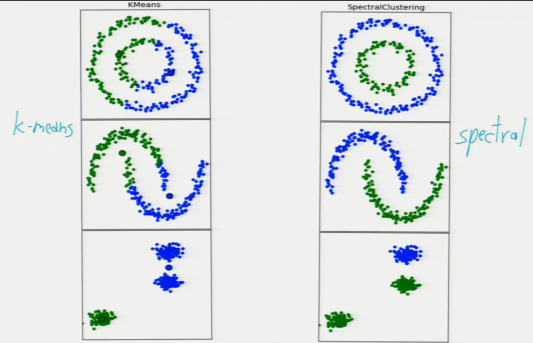
\includegraphics[scale=0.8]{../images/spectralclustering}
		\end{center}
\end{itemize}

\subsection*{Latent Factor Analysis}
\begin{itemize}
	\item Suppose $X$ is a \underline{term document matrix}: row $i$ represents document $i$; column $j$ represents term $j$.
	\item $X_{ij} = $ occurrences of term $j$ in doc $i$? better: $\log (1 + $occurrences$)$.
	\item Recall SVD $X = UDV^{T} = \sum_{i=1}^{d} \delta_{i}u_{i}u_{i}^{T}$, Suppose $\delta_{i} \leq \delta_{j}$ for $i \geq j$.
	\item For greatest $\delta_{i}$,
		\begin{itemize}
			\item each $v_{i}$ lists terms in a genre/cluster of documents.
			\item each $u_{i}$ documents using similar/relater terms.
		\end{itemize}
	\item e.g. $u_{1}$ might have large components for the romance novels, $v_{i}$ might have large components for terms "passion," "ravish," "bodice."
	\item Like clustering, but clusters overlap: if $u_{1}$ picks out romances and $u_{2}$ picks out histories, they both pick out historical romances.
	\item Application in market research: identifying consumer types (hipsters, soccer mom) and items bought together.
	\item Truncated sum $X' = \sum_{i=1}^{r} \delta_{i}u_{i}v_{i}^{T}$ is \underline{low-rank approximation}(rank r) of $X$.
		\begin{center}
			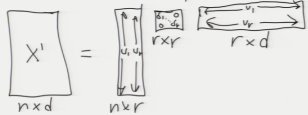
\includegraphics{../images/reducedx}
		\end{center}
		\begin{center}
			\begin{tabular}{|c|}
				\hline
				$X'$ is the rank-r matrix that minimizes Frobenium norm $||X-X'||_{F}^{2} = \sum_{i,j} (X_{ij}-X'_{ij})^{2}$\\
				\hline
			\end{tabular}
		\end{center}
	\item Applications:
		\begin{itemize}
			\item Fuzzy search.
			\item Denoising.
			\item Collaborative filtering: fills in unknown values, e.g. user ratings.
		\end{itemize}
\end{itemize}

\subsection*{Nearest Neighbor Classification}
\begin{itemize}
	\item Idea: Given query point $v$, find the $k$ input points nearest $v$. Distance metric of your choice.
	\item Regression: Return average value of the $k$ points.
	\item Classification: Return class with most votes from the $k$ points or return histogram of class probabilities.
	\item Theorem (Cover and Hart, 1967): As $n \rightarrow \infty$, the 1-NN error rate is $< B(2-B)$ where B=Bayes rate, if only 2 classes, $\leq 2B(1-B)$.
	\item Theorem (Fix and Hodges, 1951): As $n \rightarrow \infty, k \rightarrow \infty, \frac{k}{n} \rightarrow 0$, k-NN error rate converges to B.
\end{itemize}

\subsubsection*{The Geometry of High-Dimensional Spaces}
\begin{itemize}
	\item Consider unit ball $B = \{p \in \R^{d}: |p| \leq 1\}$ and hypercube $H = \{p \in \R^{d}: |p_{i}| \leq 1\}$
		\begin{center}
			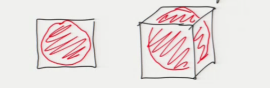
\includegraphics{../images/unitball}
		\end{center}
	\item Consider a shell of the sphere
		\begin{center}
			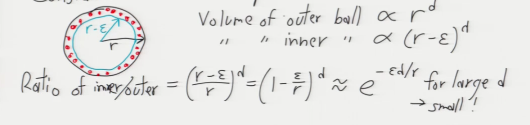
\includegraphics{../images/ell}
		\end{center}
	\item e.g. if $\frac{\epsilon}{r} = 0.1$ and d=100, inner ball has 0.0027\% of volume.
	\item Random points from (uniform$|$Gaussian) distribution in ball: nearly all are in outer shell.
\end{itemize}

\subsubsection*{Exhaustive k-NN algorithm}
\begin{itemize}
	\item Given query point $v$:
		\begin{itemize}
			\item Scan through all $n$ input points, computing (squared) distances to $v$.
			\item Maintain max-heap with the $k$ shortest distances seen so far.
		\end{itemize}
	\item Time to construct the classifier: $\bigo$
	\item Query time: $\bigo(nd + n\log k)$ expected $\bigo(nd + k\log^{2} k)$ if random point order. 
\end{itemize}

\subsubsection*{Speeding up NN}
\begin{itemize}
	\item Can we preprocess the training points to obtain sub-linear query time?
	\item Very low dimensions: Voronoi diagrams.
	\item Medium dim (up to $\sim 30$): $k-d$ trees.
	\item Larger dim: locality sensitive hashing.
	\item Largest dim: no.
	\item Usually resort to \underline{approximate} NN as $d$ gets large.
	\item Can use PCA or other dimensionality reduction as preprocess.
	\item PCA: Row $i$ of $UD$ gives the coordinates of sample point $X_{i}$ in principal components space (i.e. $X_{i}\cdot v_{j}$ for each $j$). So we don't need to project the input points onto that space; the SVD does it for us.
\end{itemize}
\end{document}










